% Physics experiment report
% 30/Sep/2016

\documentclass[a4paper,10pt,notitlepage]{report}

\usepackage{CJKutf8}
\usepackage{amsmath}
\usepackage{indentfirst}
\usepackage{graphicx}

\setlength{\parindent}{2em} 

\begin{CJK*}{UTF8}{gbsn}
\begin{document}

\title{测量元件的伏安特性曲线实验}
\author{秦光辉\ 9组3号}
\maketitle

\section*{一、实验数据处理}

	第一组数据是电流表外接法测量电阻的实验数据,表一是实验的仪器参数,表二和表三是实验中伏安数据. \\
	
\begin{table}[htbp]
\centering
	\begin{tabular}{|c|c|c|c|}
	
		\multicolumn{4}{c}{Table 1\ 实验器材参数数据表} \\
		\hline
		万用表测$R_1$ & 电压表量程($R_1$) & 电压表内阻($R_1$) & 电压表分度值($R_1$) \\
		\hline
		52.13$\Omega$ & 1.5V & 1500$\Omega$ & 0.02V \\
		\hline
		电压表等级($R_1$) & 电流表量程($R_1$) & 电流表内阻($R_1$) & 电流表分度值($R_1$) \\
		\hline
		1.0 & 30mA & 4.8$\Omega$ & 0.4mA \\
		\hline
		电流表等级($R_1$) &&& \\
		\hline
		1.0 &&& \\
		\hline
		万用表测$R_2$ & 电表短接阻值 & 电压表量程($R_2$) & 电压表内阻($R_2$) \\
		\hline
		0.9829k$\Omega$ & 0.22$\Omega$ & 7.5V & 7500$\Omega$ \\
		\hline
		电压表分度值($R_2$) & 电压表等级($R_2$) & 电流表量程($R_2$) & 电流表内阻($R_2$) \\
		\hline
		0.1V & 1.0 & 7.5mA & 16.9$\Omega$ \\
		\hline
		电流表分度值($R_1$) & 电流表等级($R_1$) &&\\
		\hline
		0.1mA & 1.0 && \\
		\hline

	\end{tabular}
\end{table}

\begin{table}[bhtp]
\centering
	\begin{tabular}{|c|c|c|c|c|c|c|c|}
	
	\multicolumn{8}{c}{Table 2\ 电流表外接法测$R_1$数据表} \\
	\hline
	U/V & 0 & 0.162 & 0.332 & 0.576 & 0.798 & 1.050 & 1.302 \\
	\hline
	I/mA & 0 & 3.16 & 6.72 & 11.64 & 16.00 & 21.12 & 26.28 \\
	\hline
	
	\end{tabular}
\end{table}

\begin{table}[bhtp]
\centering
	\begin{tabular}{|c|c|c|c|c|c|c|c|c|}
	
	\multicolumn{9}{c}{Table 3\ 电流表内接法测$R_2$数据表} \\
	\hline
	U/V & 0 & 1.10 & 2.12 & 3.38 & 4.40 & 5.46 & 6.44 & 6.97 \\
	\hline
	I/mA & 0 & 1.09 & 2.15 & 3.39 & 4.39 & 5.50 & 6.49 & 7.00 \\
	\hline
	
	\end{tabular}
\end{table}

	我用Matlab进行线性拟合,得到图1和图2所示的图线. \\
	
\begin{figure}[htbp]
\centering
	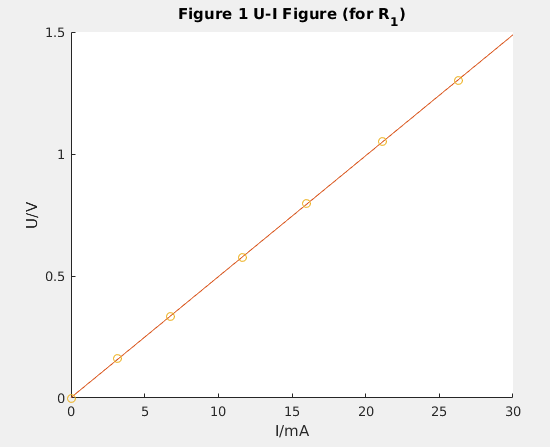
\includegraphics[scale=.45]{r1.png}
	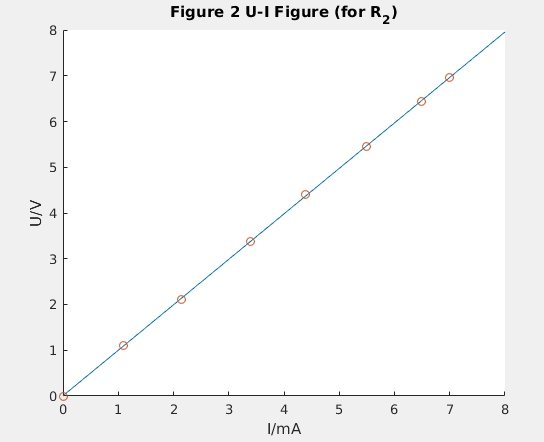
\includegraphics[scale=.45]{r2.png}
\end{figure}

	$R_1$线性回归斜率为0.0496,相关系数为0.999982.计算得其阻值为
	
\begin{equation}
	\bar{R_1}' = 49.6\Omega
\end{equation}

	考虑到观测误差和仪器误差相比小一个数量级,可以忽略掉观测误差,直接算仪器的相对误差.两个电表都是1.0级电表,故我们有
	
\begin{equation}
	\delta R_1' = R_1' * \sqrt{1\%^2 + 1\%^2} = 0.7\Omega
\end{equation}

	再把电压表分流的因素考虑在内,我们有
	
\begin{equation}
	R_1 = 51.3 \pm 0.7\Omega
\end{equation}

	万用表测得$R_1$内阻为51.92$\Omega$,我的实验数据可以覆盖这个真值. \\
	
	图线2的斜率为0.9940,相关系数为0.999976,考虑到电流表的分压和误差,我们可以计算得
	
\begin{equation}
	R_2 = 977 \pm 20 \Omega
\end{equation}

	同样覆盖了真值. \\
	
	表四是测量稳压二极管的实验数据. \\
	
\begin{table}[bhtp]
\centering
	\begin{tabular}{|c|c|c|c|c|c|c|c|c|c|}
	
	\multicolumn{9}{c}{Table 4\ 稳压二极管伏安数据表} \\
	\hline
	U/V & -5.419 & -5.408 & -5.396 & -5.383 & -5.381 & -5.373 & -5.364 & -5.343 & -5.338 \\
	\hline
	I/mA & -18.749 & -15.976 & -13.386 & -10.968 & -9.998 & -9.013 & -5.520 & -2.368 & -1.5002 \\
	\hline
	\hline
	U/V & -5.327 & -5.309 & -5.126 & -4.252 & -3.856 & -2.202 & -1.027 & 0 & 0.3774 \\
	\hline
	I/mA & -0.4350 & -0.1426 & -0.0215 & -0.0023 & -0.0013 & -0.0003 & -0.0001 & 0  & 0.000\\
	\hline
	\hline
	U/V & 0.5072 & 0.6711 & 0.7054 & 0.7262 & 0.7423 & 0.7523 & 0.7645 & 0.7739 & 0.7840 \\
	\hline
	I/mA & 0.002 & 0.066 & 0.152 & 0.260 & 0.401 & 0.525 & 0.744 & 0.975 & 1.300 \\
	\hline
	\hline
	U/V & 0.7936 & 0.7971 & 0.8000 & 0.8052 & 0.8074 & 0.8118 & 0.8202 & 0.8296 & 0.8367 \\
	\hline
	I/mA & 1.716 & 1.895 & 2.066 & 2.391 & 2.552 & 2.894 & 3.668 & 4.732 & 8.567 \\
	\hline
	
	\end{tabular}
\end{table}

	图三是稳压二极管的伏安特性曲线. \\
	
\begin{figure}
\centering
	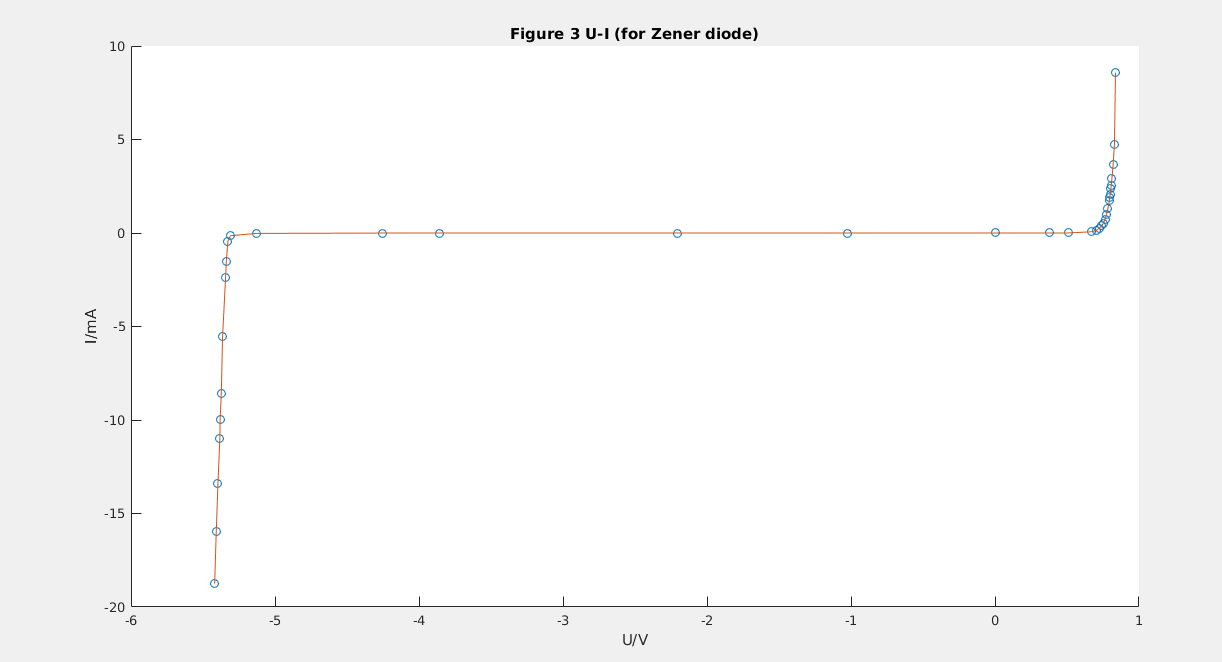
\includegraphics[scale=0.3]{diode.png}
\end{figure}

	可以计算得到二极管在-4.0V的静态电阻$r_1$,在0.8V的静态电阻$r_2$,在-10mA处的动态电阻$r_3$. \\
	
\begin{align}
	r_1 &= \frac{4.000V}{0.0015mA} = 2.7 * 10^6 \Omega \\
	r_2 &= \frac{0.8000V}{2.066mA} = 3.872 * 10^2 \Omega \\
	r_3 &= \frac{-5.373 V - (-5.396 V)}{-9.013mA - (-10.968mA)} = 1.2 * 10^2 \Omega
\end{align}

\section*{二、分析和讨论}
\subsection*{1.电流表接法分析}
	
	在考虑电压表和电流表的影响之前,两个电阻的测量值均没有覆盖真值.修正之后,考虑到系统误差,两个测量值均覆盖了真值. \\
	
	在第一个实验中,修正之前电阻是49.6$\Omega$,修正之后是51.3$\Omega$,相对误差为3.4$\%$. \\
	
	在第二个实验中,修正之前电阻是994$\Omega$,修正之后是977$\Omega$,相对误差为1.7$\%$. \\
	
	对于电流表外接,误差为
	
\begin{equation}
	\Delta R_1 = \frac{R^2}{R + R_V}
\end{equation}

	对于电流表内接,误差为
	
\begin{equation}
	\Delta R_2 = R_A
\end{equation}

	令
	
\begin{equation}
	\Delta R_1 = \Delta R_2
\end{equation}
	
	我们得到
	
\begin{equation}
	R_0 = \frac{R_A+\sqrt{R_A^2 + 4R_AR_V}}{2}
\end{equation}

	当R大于$R_0$时,我们选择电流表内接法;当R小于$R_0$时,我们选择电流表外接法.

\subsection*{2.实验测得的稳压二极管的静态,动态电阻值反映了二极管的什么特性}

	静态电阻值反映了二极管在直流电路下的阻值特性,动态电阻值反映了二极管在交流电路中的特性. \\
	
	两个静态阻值都取在了二极管尚未被完全击穿的地方.两个阻值都非常大,可见二极管在被击穿之前其阻值非常之大,以至于电流无法通过. \\
	
	动态电阻值取在了击穿的区域,其阻值非常小,说明二极管击穿之后对电流的阻碍作用就变得特别小. \\
	
\subsection*{3.使用多用表测量二极管的正向电阻,为什么不同档位测得的数值不同?如果测量一个线性电阻,结果会怎么样?}

	多用表欧姆表区域不同档位测量二极管时通过的电流也不同,不同的电流会使二极管呈现出不同的特性.二极管的伏安特性曲线不是线性的,测量的结果自然会有不同. \\
	
	如果测量对象是一个线性电阻,因为不同档位万用表的内阻不同,测量的数值也不同,但结果差异没有二极管大. \\
	
\subsection*{4.测量正向伏安曲线时使用什么电表接法?}

	电流表外接法.在测量伏安特性曲线的时候我用万用表当做电压表使用,其阻值非常大,在10M$\Omega$的量级,产生的误差极小. \\
	
	相比之下,万用表的电流档位其电阻不能完全忽略,故我没有采用电流表内接法. \\

\section*{三、感悟和收获}

	伏安特性曲线是表征材料性质的基本物理量之一,虽然我在实验中只测量了两种常见的元件的曲线,但是我也体会到了这个实验的一些要点所在.在电学实验中,我不能急躁地直接测量并记录数据,要严格按照规范操作,反复检查电路,并随时注意自己的安全.更改电路一定要按照电路图断电操作,这是一切电学实验都要遵守的规范. \\
	
	我在实验中测量了过多的数据,这些数据并不是特别有用.我认识到在记录数据之前,应该先粗测一次,获得曲线的大致形状之后再动手,这样可以避免很多浪费. \\

\end{CJK*}
\end{document}
